\documentclass[11pt]{article}
\usepackage[colorlinks=true, linkcolor=blue, citecolor=blue, backref=page]{hyperref}
\usepackage{amsmath}
\usepackage{amssymb}
\usepackage{pgfplots}
\pgfplotsset{compat=1.14}

\begin{document}

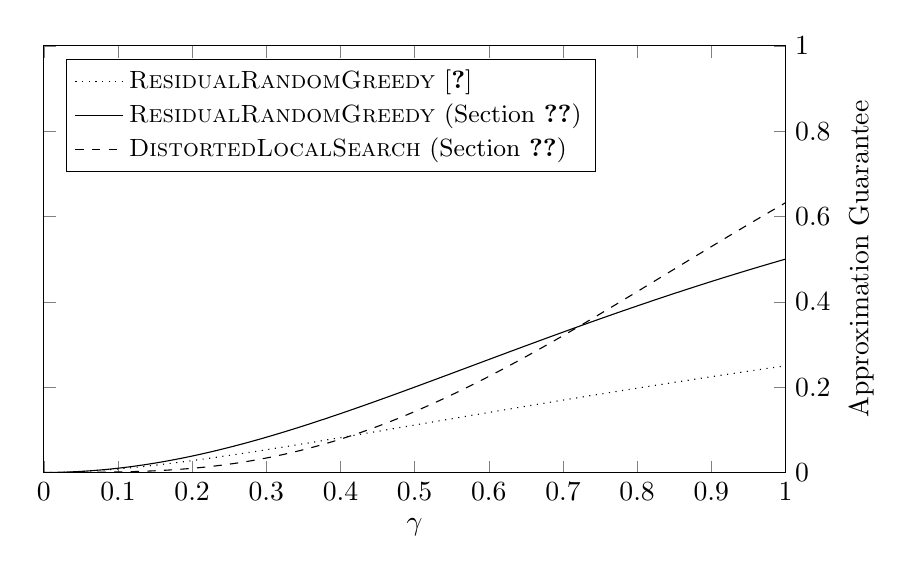
\begin{tikzpicture}
\begin{axis}[
  xlabel={$\gamma$},
  ylabel={Approximation Guarantee},
  xmin=0,
  xmax=1,
  ymin = 0,
  ymax = 1,
  legend cell align=left,
  legend pos=north west,
  ylabel  near ticks,
  yticklabel pos = right,
  width = 11cm,
  height = 7cm
]
  \addplot[domain=0:1,samples=201,dotted] {x^2/(1+x)^2};
  \addplot[domain=0:1,samples=201] {x/(x+1/x)};
  \addplot[domain=0.05:1,samples=201,dashed] {(x^3)*(1-exp(1-1/x-x^2))/(1-x+x^3)};
\legend{\small \textsc{ResidualRandomGreedy}~\cite{Chen:2018:Weakly},\small\textsc{ResidualRandomGreedy} (Section~\ref{sec:impr-analys-rrg}), \small \textsc{DistortedLocalSearch} (Section~\ref{sec:non-oblivious-local})}
\end{axis}
\end{tikzpicture}

\end{document}